\chapter{SİSTEM ANALİZİ VE FİZİBİLİTE}
\section{Sistem Analizi}
\label{sec:sistem-analizi}

Bu bölüm, modern çok ajanlı yapay zekâ metodolojilerini takip ederek ``Otonom Ajan Yaklaşımıyla Kod Veritabanından Eğitim İçeriği Üreten'' projenin kapsamını netleştirir. Amaç şekil 2.1'de gösterildiği üzere, kod tabanındaki bilgiyi dağıtık bir ajan mimarisi ile derleyip kalıcı bir Bilgi Bankası üretmek ve bu çıktıyı pedagojik değeri yüksek eğitim materyallerine dönüştürmektir.

\begin{figure}[htbp]
    \centering
    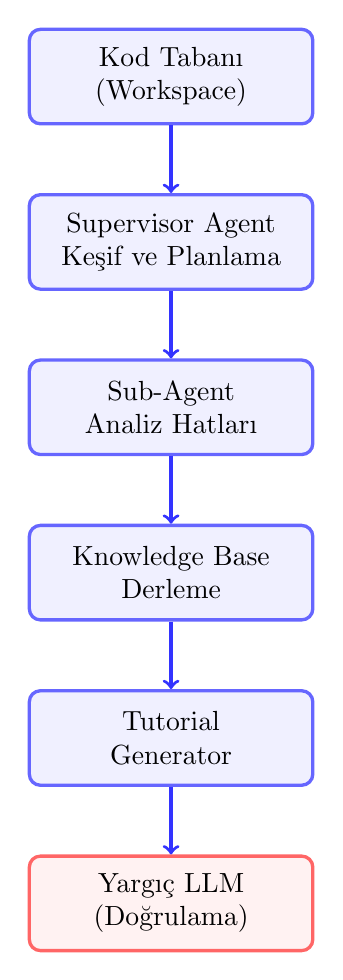
\begin{tikzpicture}[
        box/.style={rounded corners, draw=blue!60, fill=blue!6, very thick, minimum width=36mm, minimum height=12mm, align=center},
        flow/.style={->, very thick, draw=blue!80}
    ]
        \node[box] (input) at (0,0) {Kod Tabanı\\(Workspace)};
        \node[box] (analysis) at (0,-2.1) {Supervisor Agent\\Keşif ve Planlama};
        \node[box] (subpipe) at (0,-4.2) {Sub-Agent\\Analiz Hatları};
        \node[box] (kb) at (0,-6.3) {Knowledge Base\\Derleme};
        \node[box] (tutorial) at (0,-8.4) {Tutorial\\Generator};
        \node[box, fill=red!5, draw=red!60] (judge) at (0,-10.5) {Yargıç LLM\\(Doğrulama)};

        \draw[flow] (input) -- (analysis);
        \draw[flow] (analysis) -- (subpipe);
        \draw[flow] (subpipe) -- (kb);
        \draw[flow] (kb) -- (tutorial);
        \draw[flow] (tutorial) -- (judge);
    \end{tikzpicture}
    \caption{Bilgi üretim hattının üst düzey görünümü.}
    \label{fig:pipeline-overview}
\end{figure}

Mimari, iki aşamalı Sub-Agent kurgusu üzerine kuruludur. Supervisor Agent keşif, planlama ve orkestrasyon görevlerini yürütür; bağlam yükünü azaltmak için işleri Sub-Agent'lara devreder. Sub-Agent'lar kendi çalışma alanlarında ayrık olarak analiz yapar, bulgularını kalıcı depolara kaydeder ve Supervisor Agent’a raporlar. Supervisor Agent bu çıktıları birleştirerek nihai Knowledge Base'i oluşturur; ardından içerik üretimi için Tutorial Generator bileşenini tetikler.

Deterministik görev bölme yaklaşımıyla kaynak dosya altındaki ilk seviye klasörler ayrı Sub-Agent'lara atanır. Alternatif olarak Supervisor Agent, planlama parametreleri ve bir yapılacaklar listesi üzerinden görevleri dinamik biçimde güncelleyebilir. Sub-Agent'ların kod tabanına yalnızca okuma, kendi çalışma alanlarına ise yazma yetkisi vardır; böylece bağlam yönetimi ve çıktı doğrulaması sadeleşir.

\begin{figure}[htbp]
    \centering
    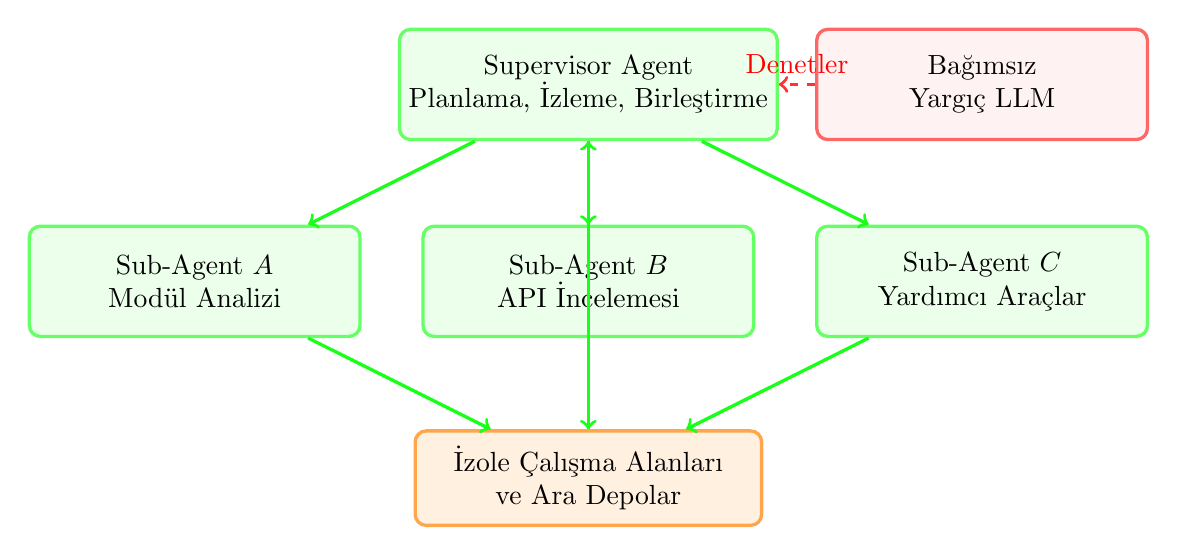
\begin{tikzpicture}[
        layer/.style={rounded corners, draw=green!60, fill=green!8, very thick, minimum width=42mm, minimum height=14mm, align=center},
        datastore/.style={rounded corners, draw=orange!70, fill=orange!12, very thick, minimum width=44mm, minimum height=12mm, align=center},
        flow/.style={->, very thick, draw=green!90}
    ]
        \node[layer] (main) at (7,4) {Supervisor Agent\\Planlama, İzleme, Birleştirme};
        \node[layer] (sub1) at (2,1.5) {Sub-Agent $A$\\Modül Analizi};
        \node[layer] (sub2) at (7,1.5) {Sub-Agent $B$\\API İncelemesi};
        \node[layer] (sub3) at (12,1.5) {Sub-Agent $C$\\Yardımcı Araçlar};
        \node[datastore] (stores) at (7,-1) {İzole Çalışma Alanları\\ve Ara Depolar};
        \node[layer, fill=red!5, draw=red!60] (judge) at (12, 4) {Bağımsız\\Yargıç LLM};

        \draw[flow] (main) -- (sub1);
        \draw[flow] (main) -- (sub2);
        \draw[flow] (main) -- (sub3);
        \draw[flow] (sub1) -- (stores);
        \draw[flow] (sub2) -- (stores);
        \draw[flow] (sub3) -- (stores);
        \draw[flow] (stores) -- (main);
        \draw[flow, dashed, draw=red!80] (judge) -- node[above, text=red]{Denetler} (main);
    \end{tikzpicture}
    \label{fig:agent-architecture}
\end{figure}


\noindent\textbf{Başarı Kriterleri ve Metrikler.}
Sistemin başarısı, teorik formüller yerine, sistem bileşenleri tarafından toplanan operasyonel veriler ve Yargıç LLM tarafından gerçekleştirilen kalite ölçümleri ile değerlendirilir.

\begin{itemize}
    \item \textbf{Operasyonel Verimlilik (Efficiency):} Sistemin bir projeyi analiz etme maliyeti şu üç temel metrikle izlenir:
    \begin{itemize}
        \item \textit{Token Tüketimi:} Toplam Girdi/Çıktı token sayısı (Maliyet analizi için).
        \item \textit{Süre (Duration):} Knowledge Base ve Tutorial fazlarının tamamlanma süreleri.
        \item \textit{Araç Kullanımı (Tool Calls):} Ajanların dosya okuma ve yazma sıklığı.
    \end{itemize}

    \item \textbf{İçerik Kalitesi (Yargıç LLM):} Üretilen eğitim içeriklerinin kalitesi, bağımsız bir LLM (Yargıç) tarafından 1-5 ölçeğinde puanlanır. Temel kriterler şunlardır:
    \begin{itemize}
        \item \textit{Doğruluk (Accuracy):} Kod örneklerinin gerçek kaynak kodla uyumu.
        \item \textit{Tamamlayıcılık (Completeness):} Konunun ne kadar kapsandığı.
        \item \textit{Pedagoji:} Anlatım sırasının mantıksal akışı.
    \end{itemize}

    \item \textbf{Süreç Dayanıklılığı (Robustness):}
    \begin{itemize}
        \item \textit{Bağlam Taşması (Context Overflow):} LLM'in hafıza sınırını aşma olaylarının sayısı.
        \item \textit{Toparlanma Başarısı:} Hata sonrası `retry` mekanizmasının başarı oranı.
    \end{itemize}
\end{itemize}


\section{Gereksinim Analizi}
\label{sec:gereksinim-analizi}

Gereksinimler üç düzeyde sınıflandırılmıştır: kullanıcı rolleri, sistem modülleri ve işlevsel akış. Sistemin iki temel kullanıcısı bulunmaktadır. Birincisi, Bilgi Bankası ve eğitim çıktıları üzerinden kod tabanını öğrenen geliştiricidir. İkincisi ise ajan süreçlerini başlatan, izleyen ve üretilen çıktının bütünlüğünü doğrulayan sistem operatörüdür. 

Sistem modülleri dört ana bileşenden oluşur. Supervisor Agent; keşif, planlama, görev dağıtımı ve Sub-Agent'lardan gelen çıktıları birleştirme görevlerini üstlenen merkezî unsurdur. Sub-Agent'lar; deterministik olarak veya koşula bağlı şekilde üretilen, belirli dizinleri veya görev kümelerini analiz eden ve izole çalışma alanlarında faaliyet gösteren ajanlardır. Knowledge Base deposu, tüm Sub-Agent özetlerinin toplandığı yapısal bir klasör düzeni sunarken, Tutorial Generator bileşeni bu Knowledge Base’i kullanarak pedagojik değer taşıyan eğitim materyallerini bağımsız bir çıktı klasörü altında üretir.

Sistemin işlevsel akışı ardışık beş aşamada gerçekleşir. İlk aşamada Supervisor Agent kod tabanının dosya yapısını çıkarır, kritik bileşenleri analiz eder ve deterministik ya da dinamik olarak görev listesini oluşturur. İkinci aşamada bu görevler ilgili Sub-Agent'lara dağıtılır. Üçüncü aşamada Sub-Agent'lar, sorumlu oldukları kod parçalarını inceleyerek özetlerini kendi çalışma dizinlerine kaydeder. Dördüncü aşamada Supervisor Agent bu alt çıktıları bir araya getirerek bütünleşik Knowledge Base’i oluşturur ve kalite kontrolünü gerçekleştirir. Son aşamada Tutorial Generator, oluşturulan bu Knowledge Base’i geliştiricilerin kolay öğrenebileceği bir pedagojik formata dönüştürür.

İşlevsel olmayan gereksinimler ise sistemin güvenlik, izlenebilirlik, genişletilebilirlik ve performans özelliklerini belirlemektedir. Sistem, özellikle dizin gezintisi (path traversal) zafiyetlerine karşı güvenli olacak şekilde tasarlanmalı; tüm API anahtarları gizli tutulmalı ve kod tabanına gömülmemelidir. Ayrıca ajanların karar verme süreçleri, özellikle görev delegasyonu  ve dosya işlemleri Phoenix aracı üzerinden ayrıntılı biçimde loglanmalıdır. Mimari, yeni araçların veya ajan türlerinin eklenmesine açık bir genişletilebilirlik sunmalıdır. Son olarak performans açısından, bir prototip olması nedeniyle süreç karmaşıklığını azaltmak amacıyla Sub-Agent'ların paralel değil, sıralı olarak çalıştırılması tercih edilmiştir.

\section{Fizibilite}
\label{sec:fizibilite}

\subsection{Teknik Fizibilite}
\label{sec:teknik-fizibilite}

\subsubsection{Donanım}
\label{sec:donanim-fizibilitesi}
Model eğitimi hedeflenmediği için yüksek donanım yatırımı gerekmez. LLM çağrıları API tabanlıdır; standart bir geliştirici bilgisayarı yeterlidir. İş yükü Sub-Agent'lara bölündüğü için bellek baskısı artmaz, uzun dosya okumaları engellenir.

\subsubsection{Yazılım}
\label{sec:yazilim-fizibilitesi}
\begin{itemize}
    \item \textbf{İşletim Sistemi:} Windows, macOS veya Linux.
    \item \textbf{Programlama Dili:} Python 3.10+ (Backend), TypeScript/React (Frontend).
    \item \textbf{Çerçeveler ve Araçlar:} \texttt{smolagents} (Ajan Orkestrasyonu), \texttt{LiteLLM} (AI Gateway), \texttt{Next.js} (Web Arayüzü), \texttt{Phoenix} (İzleme).
\end{itemize}

\subsection{Yasal Fizibilite}
\label{sec:yasal-fizibilite}
Kullanılan kütüphaneler MIT veya Apache~2.0 benzeri açık kaynak lisanslarıyla dağıtılır. Analiz edilecek kod tabanının proje ekibine ait olması veya lisans uyumunun sağlanması yeterlidir.

\subsection{Ekonomik Fizibilite}
\label{sec:ekonomik-fizibilitesi}

Projenin ekonomik fizibilitesi, düşük başlangıç maliyeti ve yüksek katma değer üretme potansiyeli sayesinde olumlu olarak değerlendirilmektedir. Sistem, büyük ölçüde açık kaynaklı yazılımlar ve bulut tabanlı LLM servisleri üzerine kurulu olup, merkezi ve sürekli bir altyapı yatırımı gerektirmemektedir.

\subsubsection{Giderler}

Temel bileşenler ücretsizdir. Maliyet kalemleri ağırlıklı olarak mühendislik eforu ve LLM API çağrılarından oluşmaktadır. Geliştirme ve test aşamalarında Google AI Studio veya OpenRouter üzerinden sunulan ücretsiz ya da düşük maliyetli modeller kullanılabilmektedir. Son kullanıcıya sunulan nihai dokümantasyon ve eğitim içeriklerinin üretiminde ise daha güçlü modeller tercih edilerek kalite–maliyet dengesi sağlanmaktadır.

Başlıca gider kalemleri aşağıda özetlenmiştir:

\begin{itemize}
    \item \textbf{Geliştirme Maliyeti:} Sistem mimarisi, çoklu ajan orkestrasyonu ve prompt mühendisliği için harcanan mühendislik eforu.
    \item \textbf{LLM API Maliyetleri:}
    \begin{itemize}
        \item \textit{Gemini 2.5 Pro:} Ortalama bir proje analizi için yaklaşık \$0.10 – \$0.50.
        \item \textit{GPT-OSS-120B:} Yüksek kalite gerektiren son tutorial üretimi aşamalarında sınırlı ve seçici kullanım.
    \end{itemize}
\end{itemize}

\subsubsection{Katma Değer}

Sistemin sağladığı katma değer, doğrudan parasal kazançtan ziyade zaman tasarrufu ve verimlilik artışı üzerinden ortaya çıkmaktadır. Bu bağlamda öne çıkan kazanımlar şunlardır:

\begin{itemize}
    \item Dokümantasyon ve proje öğrenme süreçlerinde \%80’den fazla zaman tasarrufu.
    \item Yeni geliştiricilerin projeye adaptasyon süresinin önemli ölçüde kısalması (hızlı onboarding).
    \item Kod tabanı değiştikçe ajanların yeniden çalıştırılmasıyla sürekli güncel dokümantasyon elde edilmesi.
    \item İlk kullanımda elde edilen zaman kazancı sayesinde sistemin kendi maliyetini kısa sürede amorti edebilmesi.
\end{itemize}

Bu yönleriyle proje, hem bireysel geliştiriciler hem de kurumsal yazılım ekipleri için ekonomik açıdan sürdürülebilir ve ölçeklenebilir bir çözüm sunmaktadır.

\subsection{İşgücü ve Zaman Fizibilitesi}
\label{sec:isgucu-zaman-fizibilitesi}

\textbf{Ekip:} 2 kişi (yazılım/araştırma odaklı).

\textbf{Genel Yaklaşım:} İlk sürüm için 8–12 hafta aralığında bir geliştirme süresi öngörülür. Detaylı şema şekil 2.2'de sunulmuştur.

\begin{figure}[H]
\centering
\begin{ganttchart}[
    hgrid,
    vgrid,
    x unit=0.45cm,
    y unit chart=0.6cm,
    bar height=0.45,
    bar label font=\scriptsize,
    bar/.append style={fill=gray!30},
]{1}{12}          % ← Haftalar (1–12)
    
    \gantttitle{İşgücü Gantt Şeması (12 Hafta)}{12} \\

    % Geliştirici
    \ganttgroup{Geliştirici}{1}{12} \\
    \ganttbar{Repo + Dosya Katmanı}{1}{2} \\
    \ganttbar{Sub-Agent Temelleri}{3}{4} \\
    \ganttbar{Loglama + Retry}{9}{10} \\

    % Araştırmacı
    \ganttgroup{Araştırmacı}{1}{12} \\
    \ganttbar{Knowledge Base + Şablonlar}{5}{6} \\
    \ganttbar{Eğitim Pipeline Tasarımı}{7}{8} \\

    % Ortak Görevler
    \ganttgroup{Ortak Görevler}{1}{12} \\
    \ganttbar{Sub-Agent Tasarım Konsepti}{3}{4} \\
    \ganttbar{E2E Test + Raporlama}{11}{12} \\

\end{ganttchart}
\caption{İşgücü Fizibilitesi – Rol Bazlı Gantt Şeması}
\end{figure}
